% Stick-figure cartoons for "The problem", one page each:
%   1. speed: asleep at the desk while an R loop crawls towards its end;
%   2. gradients: puzzling over the gradient of a mixed logit likelihood;
%   3. GPU: glaring at a GPU that mostly talks to Python.
% All three share a 5cm x 3.6cm bounding box, so they line up on the slide.
% Build: pdflatex problem-cartoons.tex, then
%        pdf2svg problem-cartoons.pdf problem-<name>.svg <page>
\documentclass[tikz, border=2pt]{standalone}
\usepackage[T1]{fontenc}
\usepackage{amsmath}
\renewcommand{\familydefault}{\sfdefault}
\definecolor{accent}{HTML}{107895}

\tikzset{
  ink/.style={line width=1.2pt, draw=black!80, line cap=round, line join=round},
  fine/.style={line width=0.7pt, draw=black!75, line cap=round},
  floor/.style={line width=0.8pt, draw=black!35}
}

% A GPU card centered at the origin of the current scope.
\newcommand{\gpucard}{
  \draw[ink, fill=black!5, rounded corners=2pt] (-0.9, -0.42) rectangle (0.9, 0.42);
  \foreach \x in {-0.45, 0.45} {
    \draw[fine] (\x, 0) circle (0.3);
    \draw[accent, line width=1pt] (\x, 0) circle (0.17);
    \fill[black!45] (\x, 0) circle (0.06);
  }
  \fill[black!40] (-0.65, -0.42) rectangle (0.3, -0.56);
}

% A four-pointed sparkle.
\newcommand{\sparkle}[1]{
  \draw[accent, line width=1pt, line cap=round] #1 ++(-0.11, 0) -- ++(0.22, 0);
  \draw[accent, line width=1pt, line cap=round] #1 ++(0, -0.11) -- ++(0, 0.22);
}

\begin{document}

% --- 1. speed -------------------------------------------------------------------------
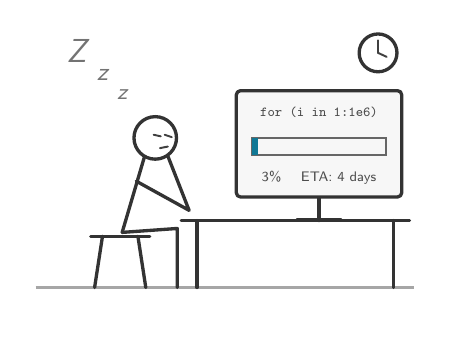
\begin{tikzpicture}
  \path[use as bounding box] (0, 0) rectangle (5, 3.6);
  \draw[floor] (0.1, 0.3) -- (4.9, 0.3);
  % desk and monitor
  \draw[ink] (1.95, 1.15) -- (4.85, 1.15);
  \draw[ink] (2.15, 1.15) -- (2.15, 0.3);
  \draw[ink] (4.65, 1.15) -- (4.65, 0.3);
  \draw[ink] (3.7, 1.15) -- (3.7, 1.45);
  \draw[ink] (3.42, 1.16) -- (3.98, 1.16);
  \draw[ink, fill=black!3, rounded corners=1.5pt] (2.65, 1.45) rectangle (4.75, 2.8);
  \node[font=\tiny\ttfamily, text=black!70] at (3.7, 2.52) {for (i in 1:1e6)};
  \draw[fine, black!60] (2.85, 1.98) rectangle (4.55, 2.2);
  \fill[accent] (2.85, 1.98) rectangle (2.92, 2.2);
  \node[font=\tiny, text=black!70] at (3.7, 1.7) {3\% \quad ETA: 4 days};
  % stool
  \draw[ink] (0.8, 0.95) -- (1.55, 0.95);
  \draw[ink] (0.95, 0.95) -- (0.85, 0.3);
  \draw[ink] (1.4, 0.95) -- (1.5, 0.3);
  % slumped figure, head propped on a hand, asleep
  \draw[ink, fill=white] (1.62, 2.2) circle (0.27);
  \draw[ink] (1.48, 1.95) -- (1.2, 1.0);
  \draw[ink] (1.2, 1.0) -- (1.9, 1.05) -- (1.9, 0.3);
  \draw[ink] (1.38, 1.65) -- (2.05, 1.28) -- (1.78, 1.97);
  \draw[fine] (1.6, 2.24) -- (1.69, 2.22);
  \draw[fine] (1.74, 2.24) -- (1.83, 2.21);
  \draw[fine] (1.68, 2.07) -- (1.78, 2.09);
  \node[font=\footnotesize\itshape, text=black!55] at (1.2, 2.75) {z};
  \node[font=\small\itshape, text=black!55] at (0.95, 3.0) {z};
  \node[font=\large\itshape, text=black!55] at (0.62, 3.3) {Z};
  % wall clock
  \draw[ink, fill=white] (4.45, 3.28) circle (0.24);
  \draw[fine] (4.45, 3.28) -- ++(90:0.16);
  \draw[fine] (4.45, 3.28) -- ++(-25:0.12);
\end{tikzpicture}

% --- 2. gradients -----------------------------------------------------------------------
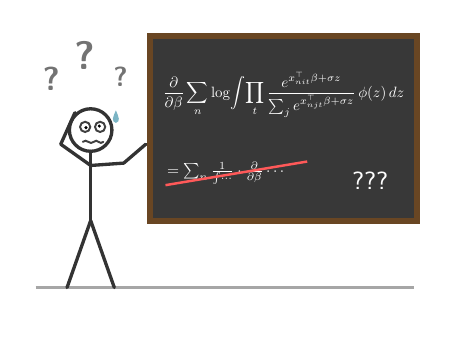
\begin{tikzpicture}
  \path[use as bounding box] (0, 0) rectangle (5, 3.6);
  \draw[floor] (0.1, 0.3) -- (4.9, 0.3);
  % chalkboard with the gradient of a mixed logit log-likelihood
  \draw[line width=2.2pt, draw=brown!55!black, fill=black!78] (1.55, 1.15) rectangle (4.95, 3.5);
  \node[text=white, scale=0.54] at (3.25, 2.75)
    {$\displaystyle \frac{\partial}{\partial \beta} \sum_{n} \log \!\int\! \prod_{t}
      \frac{e^{x_{nit}^{\top} \beta + \sigma z}}{\sum_{j} e^{x_{njt}^{\top} \beta + \sigma z}}
      \, \phi(z) \, dz$};
  \node[text=white, scale=0.56, anchor=west] at (1.7, 1.75)
    {$= \sum_{n} \frac{1}{\int \cdots} \cdot \frac{\partial}{\partial \beta} \cdots$};
  \draw[red!65, line width=0.9pt] (1.75, 1.6) -- (3.55, 1.9);
  \node[text=white, font=\small] at (4.35, 1.65) {???};
  % puzzled figure, scratching its head, chalk in the other hand
  \draw[ink, fill=white] (0.8, 2.3) circle (0.27);
  \draw[ink] (0.8, 2.03) -- (0.8, 1.15);
  \draw[ink] (0.8, 1.15) -- (0.5, 0.3);
  \draw[ink] (0.8, 1.15) -- (1.1, 0.3);
  \draw[ink] (0.8, 1.85) -- (0.42, 2.12) -- (0.6, 2.52);
  \draw[ink] (0.8, 1.85) -- (1.22, 1.88) -- (1.5, 2.12);
  \draw[fine, fill=white] (0.73, 2.34) circle (0.065);
  \draw[fine, fill=white] (0.92, 2.34) circle (0.065);
  \fill[black] (0.74, 2.33) circle (0.022);
  \fill[black] (0.91, 2.35) circle (0.022);
  \draw[fine] (0.7, 2.15) .. controls (0.75, 2.2) and (0.79, 2.1) .. (0.84, 2.15)
    .. controls (0.88, 2.2) and (0.92, 2.1) .. (0.96, 2.15);
  \fill[accent!55] (1.12, 2.55) .. controls (1.08, 2.46) and (1.06, 2.41) .. (1.12, 2.39)
    .. controls (1.18, 2.41) and (1.16, 2.46) .. (1.12, 2.55);
  \node[font=\large\bfseries, text=black!55] at (0.3, 2.95) {?};
  \node[font=\Large\bfseries, text=black!55] at (0.72, 3.25) {?};
  \node[font=\normalsize\bfseries, text=black!55] at (1.18, 2.98) {?};
\end{tikzpicture}

% --- 3. GPU ----------------------------------------------------------------------------
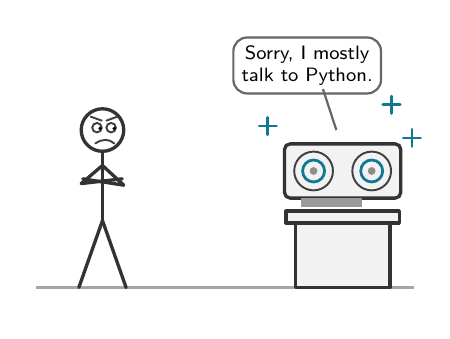
\begin{tikzpicture}
  \path[use as bounding box] (0, 0) rectangle (5, 3.6);
  \draw[floor] (0.1, 0.3) -- (4.9, 0.3);
  % a GPU on a pedestal, sparkling
  \draw[ink, fill=black!5] (3.4, 0.3) rectangle (4.6, 1.12);
  \draw[ink, fill=black!5] (3.28, 1.12) rectangle (4.72, 1.27);
  \begin{scope}[shift={(4.0, 1.78)}, scale=0.82]
    \gpucard
  \end{scope}
  \sparkle{(3.05, 2.35)}
  \sparkle{(4.88, 2.2)}
  \sparkle{(4.62, 2.62)}
  \node[draw=black!60, line width=0.8pt, fill=white, rounded corners=5pt, font=\scriptsize,
    align=center, inner sep=3pt] (talk) at (3.55, 3.12) {Sorry, I mostly\\talk to Python.};
  \draw[black!60, line width=0.8pt] (3.75, 2.82) -- (3.92, 2.3);
  % jealous figure: arms crossed, eyes sideways at the GPU, frowning
  \draw[ink, fill=white] (0.95, 2.3) circle (0.27);
  \draw[ink] (0.95, 2.03) -- (0.95, 1.15);
  \draw[ink] (0.95, 1.15) -- (0.65, 0.3);
  \draw[ink] (0.95, 1.15) -- (1.25, 0.3);
  \draw[ink] (0.95, 1.85) -- (0.68, 1.62) -- (1.2, 1.68);
  \draw[ink] (0.95, 1.85) -- (1.22, 1.6) -- (0.7, 1.68);
  \draw[fine, fill=white] (0.88, 2.33) circle (0.06);
  \draw[fine, fill=white] (1.06, 2.33) circle (0.06);
  \fill[black] (0.92, 2.32) circle (0.024);
  \fill[black] (1.1, 2.32) circle (0.024);
  \draw[fine] (0.8, 2.47) -- (0.94, 2.42);
  \draw[fine] (1.0, 2.42) -- (1.14, 2.47);
  \draw[fine] (0.86, 2.13) .. controls (0.95, 2.19) and (1.03, 2.19) .. (1.1, 2.13);
\end{tikzpicture}

\end{document}
